\documentclass{article}
\usepackage{amsfonts} % For open face letters
\usepackage{amsmath} % For align*
\usepackage{graphicx} % For images
\usepackage{enumitem} % For customisable list labels
\graphicspath{{./images/}}

\renewcommand{\vec}[1]{\boldsymbol{\mathbf{#1}}}
\newcommand{\dvec}[1]{\dot{\vec{#1}}}
\newcommand{\ddvec}[1]{\ddot{\vec{#1}}}
\newcommand{\uvec}[1]{\hat{\vec{#1}}}

\newcommand{\ke}{\frac{1}{4 \pi \epsilon_0}}

\def\rcurs{{\mbox{$\resizebox{.09in}{.08in}{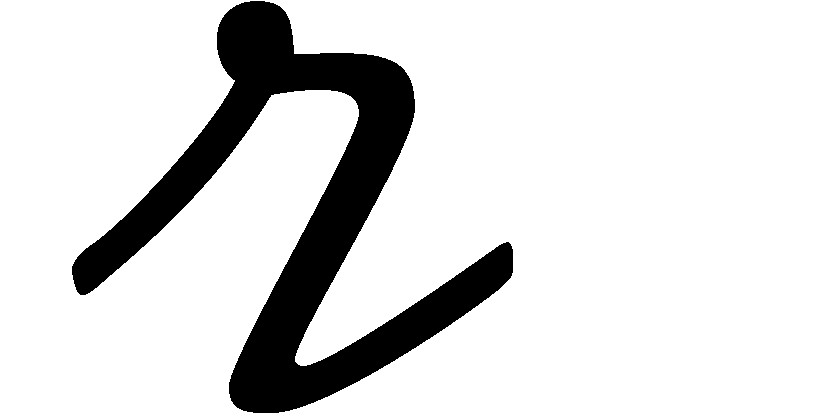
\includegraphics[trim= 1em 0 14em 0,clip]{ScriptR}}$}}}
\def\brcurs{{\mbox{$\resizebox{.09in}{.08in}{
\includegraphics[trim= 1em 0 14em 0,clip]{BoldR}}$}}}
\def\hrcurs{{\mbox{$\hat \brcurs$}}}

\setlist[enumerate, 1]{label={(\alph*)}}
\setlist[enumerate, 2]{label={(\roman*)}}

\title{Introduction to Electrodynamics by David J. Griffiths Problems}
\author{Chris Doble}
\date{December 2023}

\begin{document}

\maketitle

\tableofcontents

\setcounter{section}{1}
\section{Electrostatics}

\subsection{}

\begin{enumerate}
  \item $\vec{0}$

  \item The same as if only the opposite charge were present — all others are cancelled out.
\end{enumerate}

\subsection{}

\begin{align*}
  \vec{E} & = \ke 2 \frac{q}{\rcurs^2} \cos \theta \uvec{x}      \\
          & = \ke \frac{d q}{[(d / 2)^2 + z^2]^{3 / 2}} \uvec{x}
\end{align*}

\subsection{}

\begin{align*}
  \vec{r}  & = z \uvec{z}                                                                                                                          \\
  \vec{r}' & = x \uvec{x}                                                                                                                          \\
  \brcurs  & = z \uvec{z} - x \uvec{x}                                                                                                             \\
  \rcurs   & = \sqrt{x^2 + z^2}                                                                                                                    \\
  \hrcurs  & = \frac{z \uvec{z} - x \uvec{x}}{\sqrt{x^2 + z^2}}                                                                                    \\
  \vec{E}  & = \ke \int_0^L \frac{\lambda}{x^2 + z^2} \frac{z \uvec{z} - x \uvec{x}}{\sqrt{x^2 + z^2}} \,d x                                       \\
           & = \ke \lambda \left( z \uvec{z} \int_0^L \frac{1}{(x^2 + z^2)^{3 / 2}} \,d x - \uvec{x} \int_0^L \frac{x}{(x^2 + z^2)} \,d x \right)  \\
           & = \ke \lambda \left[ \frac{L}{z \sqrt{L^2 + z^2}} \uvec{z} - \left( \frac{1}{z} - \frac{1}{\sqrt{L^2 + z^2}} \right) \uvec{x} \right] \\
           & = \ke \frac{\lambda}{z} \left[ \left( -1 + \frac{z}{\sqrt{L^2 + z^2}} \right) \uvec{x} + \frac{L}{\sqrt{L^2 + z^2}} \uvec{z} \right]
\end{align*}

\subsection{}

The electric field a distance $z$ above the midpoint of a line segment of length $2 L$ and uniform line charge $\lambda$ is \[\vec{E} = \ke \frac{2 \lambda L}{z \sqrt{z^2 + L^2}} \uvec{z}.\]

Applying this to the four sides of the square, the horizontal components of opposite sides cancel leaving only the vertical component.

\begin{align*}
  \cos \theta & = \frac{z}{\rcurs}                                                                                                      \\
              & = \frac{z}{\sqrt{(a / 2)^2 + z^2}}                                                                                      \\
  \vec{E}     & = 4 \left( \ke \frac{\lambda a}{\sqrt{(a / 2)^2 + z^2} \sqrt{(a / 2)^2 + (a / 2)^2 + z^2}} \uvec{z} \right) \cos \theta \\
              & = \ke \frac{4 a \lambda z}{[(a / 2)^2 + z^2] \sqrt{(a^2 / 2) + z^2}} \uvec{z}
\end{align*}

\subsection{}

\begin{align*}
  \vec{E} & = \ke \int_0^{2 \pi} \frac{\lambda r}{r^2 + z^2} \cos \alpha \,d \theta \,\uvec{z} \\
          & = \ke \frac{2 \pi \lambda r z}{(r^2 + z^2)^{3 / 2}} \uvec{z}
\end{align*}

\subsection{}

\begin{align*}
  \vec{E} & = \ke \int \frac{d q}{\rcurs^2} \cos \theta \uvec{z}                                                          \\
          & = \ke \int_0^{2 \pi} \int_0^R \frac{\sigma}{r^2 + z^2} \frac{z}{\sqrt{r^2 + z^2}} r \,d r \,d \theta \uvec{z} \\
          & = \ke 2 \pi \sigma z \int_0^R \frac{r}{(r^2 + z^2)^{3 / 2}} \,d r \,\uvec{z}                                  \\
          & = \ke 2 \pi \sigma z \left( \frac{1}{z} - \frac{1}{\sqrt{R^2 + z^2}} \right) \uvec{z}
\end{align*}

When $R \rightarrow \infty$ \[\vec{E} = \frac{\sigma}{2 \epsilon_0} \uvec{z}.\]

\subsection{}

\[\vec{E} = \begin{cases}
    \ke \frac{q}{z^2} \uvec{z} & z > R \\
    \vec{0}                    & z < R
  \end{cases}\]

\subsection{}

\[\vec{E} = \begin{cases}
    \ke \frac{q}{z^2} \uvec{z}   & z > R \\
    \ke \frac{q z}{R^3} \uvec{z} & z < R
  \end{cases}\]

\subsection{}

\begin{enumerate}
  \item

        \begin{align*}
          \rho & = \epsilon_0 \nabla \cdot \vec{E}                              \\
               & = \epsilon_0 \frac{1}{r^2} \frac{\partial}{\partial r} (k r^5) \\
               & = 5 \epsilon_0 k r^2
        \end{align*}

  \item

        \begin{align*}
          Q_\text{enc} & = \epsilon_0 \oint \vec{E} \cdot d \vec{a}                                                        \\
                       & = \epsilon_0 \int_0^{2 \pi} \int_0^\pi k R^3 R \,d \theta R \sin \theta \,d \phi                  \\
                       & = 2 \pi \epsilon_0 k R^5 [-\cos \theta]_0^\pi                                                     \\
                       & = 4 \pi \epsilon_0 k R^5                                                                          \\
          Q_\text{enc} & = \int_V \rho \,d \tau                                                                            \\
                       & = \int_0^{2 \pi} \int_0^\pi \int_0^R 5 \epsilon_0 k r^2 \,d r r \,d \theta r \sin \theta \,d \phi \\
                       & = 10 \pi \epsilon_0 k \int_0^\pi \int_0^R r^4 \sin \theta \,d r \,d \theta                        \\
                       & = 2 \pi \epsilon_0 k R^5 [-\cos \theta]_0^\pi                                                     \\
                       & = 4 \pi \epsilon_0 k R^5
        \end{align*}
\end{enumerate}

\subsection{}

If the charge was surrounded by $8$ such cubes the total flux through all the cubes would be $q / \epsilon_0$. There are $24$ outside faces to the larger cube, so the total flux through the shaded face is $q / (24 \epsilon_0)$.

\subsection{}

\begin{align*}
  \int \vec{E}_\text{inside} \cdot d \vec{a}  & = \frac{Q_\text{enc}}{\epsilon_0}     \\
                                              & = 0                                   \\
  \vec{E}_\text{inside}                       & = \vec{0}                             \\
  \int \vec{E}_\text{outside} \cdot d \vec{a} & = \frac{Q_\text{enc}}{\epsilon_0}     \\
  4 \pi r^2 E_\text{outside}                  & = \frac{4 \pi R^2 \sigma}{\epsilon_0} \\
  \vec{E}_\text{outside}                      & = \ke \frac{q}{r^2} \uvec{r}
\end{align*}

\subsection{}

\begin{align*}
  \int \vec{E} \cdot d \vec{a} & = \frac{Q_\text{enc}}{\epsilon_0}             \\
  4 \pi r^2 E                  & = \frac{\frac{4}{3} \pi r^3 \rho}{\epsilon_0} \\
  \vec{E}                      & = \frac{r \rho}{3 \epsilon_0} \uvec{r}
\end{align*}

\subsection{}

\begin{align*}
  \int \vec{E} \cdot d \vec{a} & = \frac{Q_\text{enc}}{\epsilon_0}                       \\
  2 \pi s l E                  & = \frac{l \lambda}{\epsilon_0}                          \\
  \vec{E}                      & = \frac{1}{2 \pi \epsilon_0} \frac{\lambda}{s} \uvec{s}
\end{align*}

\subsection{}

\begin{align*}
  Q_\text{enc}                 & = \int_V \rho \,d \tau                                                             \\
                               & = \int_0^{2 \pi} \int_0^\pi \int_0^r k r'^3 \sin \theta \,d r' \,d \theta \,d \phi \\
                               & = 2 \pi k \int_0^\pi \left[ \frac{1}{4} r'^4 \sin \theta \right]_0^r \,d \theta    \\
                               & = \frac{1}{2} \pi k r^4 [-\cos \theta]_0^\pi                                       \\
                               & = \pi k r^4                                                                        \\
  \int \vec{E} \cdot d \vec{a} & = \frac{Q_\text{enc}}{\epsilon_0}                                                  \\
  4 \pi r^2 E                  & = \frac{\pi k r^4}{\epsilon_0}                                                     \\
  \vec{E}                      & = \frac{k r^2}{4 \epsilon_0} \uvec{r}
\end{align*}

\subsection{}

\begin{enumerate}
  \item $\vec{E} = \vec{0}$

  \item

        \begin{align*}
          Q_\text{enc} & = \int_0^{2 \pi} \int_0^\pi \int_a^r k \sin \theta \,d r' \,d \theta \,d \phi \\
                       & = 4 \pi k (r - a)                                                             \\
          4 \pi r^2 E  & = \frac{4 \pi k (r - a)}{\epsilon_0}                                          \\
          \vec{E}      & = \frac{k (r - a)}{\epsilon_0 r^2} \uvec{r}
        \end{align*}

  \item $\vec{E} = \frac{k (b - a)}{\epsilon_0 r^2} \uvec{r}$
\end{enumerate}

\subsection{}

\begin{enumerate}
  \item

        \begin{align*}
          Q_\text{enc} & = \pi s^2 l \rho                       \\
          2 \pi s l E  & = \frac{\pi s^2 l \rho}{\epsilon_0}    \\
          \vec{E}      & = \frac{s \rho}{2 \epsilon_0} \uvec{s}
        \end{align*}

  \item \[\vec{E} = \frac{a^2 \rho}{2 \epsilon_0 s} \uvec{s}\]

  \item \[\vec{E} = \vec{0}\]
\end{enumerate}

\subsection{}

\begin{align*}
  2 A E_\text{inside}   & = \frac{2 A y \rho}{\epsilon_0}           \\
  \vec{E}_\text{inside} & = \frac{y \rho}{\epsilon_0}               \\
  \vec{E}               & = \begin{cases}
                              \frac{d \rho}{\epsilon_0}  & d < y      \\
                              \frac{y \rho}{\epsilon_0}  & 0 < y < d  \\
                              -\frac{y \rho}{\epsilon_0} & -d < y < 0 \\
                              -\frac{d \rho}{\epsilon_0} & y < -d
                            \end{cases}
\end{align*}

\subsection{}

The electric field inside a uniformly charged solid sphere is \[\vec{E} = \frac{r \rho}{3 \epsilon_0} \uvec{r}.\]

\begin{align*}
  \vec{d} & = \vec{r}_1 - \vec{r}_2                                                               \\
  \vec{E} & = \frac{r_1 \rho}{3 \epsilon_0} \uvec{r}_1 - \frac{r_2 \rho}{3 \epsilon_0} \uvec{r}_2 \\
          & = \frac{\rho}{3 \epsilon_0} (\vec{r}_1 - \vec{r}_2)                                   \\
          & = \frac{\rho}{3 \epsilon_0} \vec{d}
\end{align*}

\setcounter{subsection}{19}
\subsection{}

a is impossible because its curl is nonzero.

\begin{align*}
  V         & = -\int_0^y 2 k x y' \,d y' - \int_0^z 2 k y z' \,d z                                    \\
            & = -2 k x \left[ \frac{1}{2} y'^2 \right]_0^y - 2 k y \left[ \frac{1}{2} z'^2 \right]_0^z \\
            & = -k (x y^2 + y z^2)                                                                     \\
  -\nabla V & = k [y^2 \uvec{x} + (2 x y + z^2) \uvec{y} + 2 y z \uvec{z}]                             \\
            & = \vec{E}
\end{align*}

\subsection{}

\begin{align*}
  \vec{E}                  & = \begin{cases}
                                 \ke \frac{q}{r^2}   & r > R \\
                                 \ke \frac{q r}{R^3} & r < R
                               \end{cases}                                                                    \\
  V_\text{outside}(r)      & = -\int_\infty^r \ke \frac{q}{r'^2} \,d r'                                                       \\
                           & = -\ke q \left[ -\frac{1}{r'} \right]_\infty^r                                                   \\
                           & = \ke \frac{q}{r}                                                                                \\
  -\nabla V_\text{outside} & = \ke \frac{q}{r^2} \uvec{r}                                                                     \\
                           & = \vec{E}_\text{outside}                                                                         \\
  V_\text{inside}(r)       & = -\left( \int_\infty^R \ke \frac{q}{r'^2} \,d r' + \int_R^r \ke \frac{q r'}{R^3} \,d r' \right) \\
                           & = -\left( -\ke \frac{q}{R} + \ke \frac{q}{R^3} \left[ \frac{1}{2} r'^2 \right]_R^r \right)       \\
                           & = \ke \frac{q}{2 R} \left[ 3 - \left( \frac{r}{R} \right)^2 \right]                              \\
  -\nabla V_\text{inside}  & = \ke \frac{q r}{R^3} \uvec{r}                                                                   \\
                           & = \vec{E}_\text{inside}
\end{align*}

\subsection{}

\begin{align*}
  \vec{E}   & = \frac{1}{2 \pi \epsilon_0} \frac{\lambda}{s} \uvec{s}          \\
  V         & = -\int_O^s \frac{1}{2 \pi \epsilon_0} \frac{\lambda}{s'} \,d s' \\
            & = -\frac{1}{2 \pi \epsilon_0} \lambda \ln \frac{s}{O}            \\
  -\nabla V & = \frac{1}{2 \pi \epsilon_0} \frac{\lambda}{s} \uvec{s}
\end{align*}

\subsection{}

\begin{align*}
  \vec{E} & = \begin{cases}
                \vec{0}                                   & r < a     \\
                \frac{k (r - a)}{\epsilon_0 r^2} \uvec{r} & a < r < b \\
                \frac{k (b - a)}{\epsilon_0 r^2} \uvec{r} & b < r
              \end{cases}                                                                                           \\
  V(0)    & = -\int_\infty^0 E \,d r                                                                                                                          \\
          & = -\left( \int_\infty^b \frac{k (b - a)}{\epsilon_0 r^2} \,d r + \int_b^a \frac{k (r - a)}{\epsilon_0 r^2} \,d r \right)                          \\
          & = -\left( \frac{k (b - a)}{\epsilon_0} \left[ -\frac{1}{r} \right]_\infty^b + \frac{k}{\epsilon_0} \left[ \ln r + \frac{a}{r} \right]_b^a \right) \\
          & = -\left[ -\frac{k (b - a)}{\epsilon_0 b} + \frac{k}{\epsilon_0} \left( \ln a + 1 - \ln b - \frac{a}{b} \right) \right]                           \\
          & = -\frac{k}{\epsilon_0} \left( -1 + \frac{a}{b} + \ln \frac{a}{b} + 1 - \frac{a}{b} \right)                                                       \\
          & = \frac{k}{\epsilon_0} \ln \frac{b}{a}
\end{align*}

\subsection{}

\begin{align*}
  V(b) - V(0) & = -\int_0^b E \,d r                                                                                                            \\
              & = -\left( \int_0^a \frac{s \rho}{2 \epsilon_0} \,d s + \int_a^b \frac{a^2 \rho}{2 \epsilon_0 s} \,d s \right)                  \\
              & = -\left( \frac{\rho}{2 \epsilon_0} \left[ \frac{1}{2} s^2 \right]_0^a + \frac{a^2 \rho}{2 \epsilon_0} \ln \frac{b}{a} \right) \\
              & = -\left( \frac{a^2 \rho}{4 \epsilon_0} + \frac{a^2 \rho}{2 \epsilon_0} \ln \frac{b}{a} \right)                                \\
              & = -\frac{a^2 \rho}{4 \epsilon_0} \left( 1 + 2 \ln \frac{a}{b} \right)
\end{align*}

\subsection{}

\begin{enumerate}
  \item \[V = \ke \frac{2 q}{\sqrt{(d / 2)^2 + z^2}}\]

  \item

        \begin{align*}
          V & = \ke \int_{-L}^L \frac{\lambda}{\sqrt{x^2 + z^2}} \,d x                    \\
            & = \ke \lambda \ln \left( 1 + \frac{2 L (L + \sqrt{L^2 + z^2})}{z^2} \right)
        \end{align*}

  \item

        \begin{align*}
          V & = \ke \int_0^{2 \pi} \int_0^R \frac{\sigma}{\sqrt{r^2 + z^2}} r \,d r \,d \theta \\
            & = \ke 2 \pi \sigma (\sqrt{R^2 + z^2} - z)
        \end{align*}
\end{enumerate}

\subsection{}

\begin{align*}
  V_\text{bottom}                & = \ke \int_0^{2 \pi} \int_0^h \frac{\sqrt{2} \sigma z}{\sqrt{2} z} \,d \phi \,d z             \\
                                 & = \frac{\sigma h}{2 \epsilon_0}                                                               \\
  V_\text{top}                   & = \ke \int_0^{2 \pi} \int_0^h \frac{\sqrt{2} \sigma z}{\sqrt{z^2 + (h - z)^2}} \,d \phi \,d z \\
                                 & = \frac{\sqrt{2} \sigma}{2 \epsilon_0} \int_0^h \frac{z}{\sqrt{z^2 + (h - z)^2}} \,d z        \\
                                 & = \frac{\sigma h}{4 \epsilon_0} \ln (3 + 2 \sqrt{2})                                          \\
  V_\text{bottom} - V_\text{top} & = \frac{\sigma h}{2 \epsilon_0} \left[ 1 - \frac{1}{2} \ln (3 + 2 \sqrt{2}) \right]           \\
\end{align*}

\setcounter{subsection}{27}
\subsection{}

\begin{align*}
  V(r) & = \ke \int_0^{2 \pi} \int_0^\pi \int_0^R \frac{\rho r'^2 \sin \theta}{\sqrt{r^2 + r'^2 - 2 r r' \cos \theta}} \,d r' \,d \theta \,d \phi \\
       & = \frac{\rho}{2 \epsilon_0} \int_0^\pi \int_0^R \frac{r'^2 \sin \theta}{\sqrt{r^2 + r'^2 - 2 r r' \cos \theta}} \,d r' \,d \theta        \\
       & = \frac{\rho}{2 \epsilon_0} \left( R^2 - \frac{r^2}{3} \right)                                                                           \\
       & = \frac{q}{8 \pi \epsilon_0 R} \left( 3 - \frac{r^2}{R^2} \right)
\end{align*}

\end{document}